\documentclass[10pt]{article}
\usepackage{amsfonts}
\usepackage{amsmath}
\usepackage{geometry}
\usepackage[pdftex]{graphicx}
\usepackage{subfigure}
\usepackage{multirow}
\usepackage{longtable}
\usepackage{float}
\usepackage{fullpage}
\usepackage{eucal}
\parindent=0cm

\usepackage[ruled,vlined]{algorithm2e}
\usepackage{xcolor}
\usepackage{hyperref}

\graphicspath{{images/}}

\begin{document}

\begin{minipage}{0.7\textwidth}

{\LARGE \textsc{Documentation}}

{\Large \textbf{2D Mixed--element mesh generator}

{\large Version 2018.11.23 \textsc{roi}--type}}

{\large Claudio Lobos}

\small \texttt{clobos@inf.utfsm.cl}\\
\small Departmento de Inform\'atica -- \textsc{utfsm}  -- Chile.

{\large Fabrice Jaillet}

\small \texttt{fabrice.jaillet@univ-lyon1.fr}\\
\small Universit\'e de Lyon, IUT Lyon~1 -- LIRIS CNRS UMR-5205  -- France.
\end{minipage}
\hfill
\begin{minipage}{0.28\textwidth}

\includegraphics[width=\textwidth]{utfsm-all-oc.pdf}

\includegraphics[width=\textwidth]{logo_liris_160_0.png}
\end{minipage}

\vspace{0.5cm}

\begin{abstract}
This document will show you how to obtain mixed--elements meshes with the provided code. Two main alternatives are explained here. The first will show you how to use the code as a standalone program. The second will show you how to bundle your own code with the mixed-element mesh generator. In both cases, mixed--element are employed to manage transitions between fine and coarse regions and at the boundary of the domain. All the remaining regions will be meshed with structured regular quadrangles.
\end{abstract}


%---------------------------
%---------------------------
\section{Data Structures and initialisation}
\label{sec:dataStruct}
%---------------------------
%---------------------------

\textcolor{red}{Quadrant, QuadEdge, Polyline}
\textcolor{red}{Final resulting Mesh}


This mesh generator will allow you to create a mixed--element mesh starting from a boundary 2D mesh  (polyline) composed of edges (Fig.~\ref{f:polyline}). Let this input surface mesh be $\mathcal{S}$. Two constraints must be fulfilled by $\mathcal{S}$: it must be unfolded (no self--intersection), and the normal of the edges must be pointing outside.

The algorithm will use $\mathcal{S}$ for two purposes: to find out if a point is inside or outside the domain and to project a point onto $\mathcal{S}$. Therefore, if you have two different meshes representing the exact same domain, you should use the one with less edges. The algorithm will compute faster the output mesh.

The first step of the algorithm is to compute the Bounding box (Bbox) of $\mathcal{S}$. This Bbox will not necessarily be a perfect square. Therefore, an algorithm will be employed to automatically compute a set of squares containing $\mathcal{S}$ (Fig.~\ref{f:grid}).

Now it is possible to introduce the other important input: the Refinement Level (\textit{rl}). This mesh generator is based on the  Quadtree technique introduced in \cite{Finkel1974}. This technique recursively split a Quadant in a finite number of equivalent sons. For instance if the Quadrant is a square, to refine it one level means that it will be replaced by 4 new QUadrants. All of them will be sons of the replaced Quadrant in the Quadtree structure. By allowing the use of quadrants with cut corners, this modeling technique overcomes some of the drawbacks of standard Quadtree encoding for finite element mesh generation \cite{Yerry1983}.
In our case, Quadrants will continue to refine until a maximum provided level is reached. Quadrants lying completely outside $\mathcal{S}$ will be removed.\\

 \begin{figure}[htb]
\centering
 \subfigure[~]{
  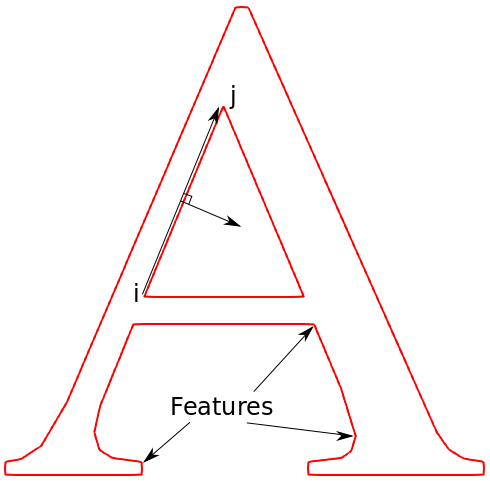
\includegraphics[width=0.24\textwidth]{a_polyline_info.png}
  \label{f:polyline}}
 \subfigure[~]{
  
\includegraphics[width=0.72\textwidth]{a_grid.png}
  \label{f:grid}}
\label{fig:boundary}
\caption{ (a) An example of complex polyline with holes and sharp features. This corresponds to the Input to be meshed (\href{https://github.com/jaillet/MixedQuadTree/blob/master/data/a.poly}{source: a.poly}) . (b) The embedding (poorly defined...) initial quadrants }
\end{figure}

%---------------------------
\subsection {Polyline as Input boundary}

A \textbf{Polyline} is composed of (Fig.~\ref{f:polyline}):
\begin{itemize}
\item a vector of  \textbf{3DPoint}, with coordinates, that are all lying inside the \textbf{BoundingBox} of the Polyline,
\item and their associated angle. If the angle is not lying in the range $[MinAngle=175,MaxAngle=185]$, then it's considered as a sharp point, and called  a \textbf{Feature} in the remaining.
\item a vector of \textbf{PolyEdge}, each one defined by the indexes of the extremity' nodes, and a normal. By convention, the normal is not normed and is pointing out the Input. For an oriented edge $(i,j)$, its right side will be outside and its left side inside. Thus, the Input must be defined by closed sets of connecting edges with counter-clockwise orientation. This way, holes may be simply created.
\end{itemize}
The format for Input file might be either \verb?.poly? as described on the \href{https://www.cs.cmu.edu/~quake/triangle.poly.html}{ Triangle\_1.6 website}; find an example here: \href{https://github.com/jaillet/MixedQuadTree/blob/master/data/unit\_square.poly}{unit\_square.poly}.
It could also be defined as \verb?.mdl? file, see \href{https://github.com/jaillet/MixedQuadTree/blob/master/data/unit\_square.mdl}{unit\_square.mdl}:

%---------------------------
\subsection{Quadrant as support of surface mesh}

The other important structure is the \textbf{Quadrant}:
\begin{itemize}
\item is composed of a \textit{pointindex}, vector of 4 corner indices in a vector of \textbf{MeshPoint}: Note here that MeshPoint is embedding a previously seen \textbf{3DPoint}, as well as some information describing its state. More details below.
\item When the Quadrant is subdived into non quadrant elements (in Transitions for example), it contains a vector of \textit{sub\_elements}, each one described by a vector of indices as presented right above.
\item It also contains a list of intersecting \textbf{PolyEdges}, and intersecting \textbf{Features}. These informations are useful to speed up the inside/outside descrimination for the Quadrant or to better handle the boundary and surface elements, for example.
\item and some additional data, for processing purpose that will be described later.
\end{itemize}

Along with the Quadrant, comes the \textbf{QuadEdge}:
\begin{itemize}
\item defined by 3 indices, the 2 extremities and potential \textit{midpoint} when this edge is split.
\end{itemize}

And finally, the \textbf{MeshPoint}:
\begin{itemize}
\item that is embedding a 3DPoint, as coordinates of the Quadrant's corners, referenced as indices.
\item MeshPoint are conversely connected to Quadrant by an index map of \textit{elements}, referencing all the Quadrants having this point as corner.
\item it also is the support for some crucial processing information on it's \textit{state}, merged in a single byte: the point is \verb?inside?, has been \verb?projected?, is representing a \verb?feature?, has been previously \verb?checked?, etc\ldots  
\end{itemize}

These three structures will be used together along with the Polyline by the \textbf{Mesher}, that will construct them gradually:
\begin{itemize}
\item a vector of \textbf{MeshPoint},
\item a vector of \textbf{Quadrant},
\item a set of \textbf{QuadEdge}. Note that this kind of structure is costly (quasi 30\% of the whole computation time), as insertion is done in a sorted container, but it guarantees uniqueness of the element, and reasonably fast access. By the way, it might not be exactly dapted to parallelism...
\item It also contains a list of \textbf{Refinement Regions}, which usage will be presented later on.
\end{itemize}

%---------------------------
%---------------------------
\section{Main steps of the method}
\label{sec:method}
%---------------------------
%---------------------------

mixed-elements mesh generation, describe here the main steps of the method

\subsection{A quadtree-based method}
show different steps of the method: 

\begin{algorithm}[H]
\SetAlgoLined
\KwResult{A mixed-elements mesh}
 \nl \ForEach{Quadrant}{
 \Repeat {desired Refinement Level}{
 \nl Subdivide Quadrant\;
   \ForEach{ new Sub-Quadrant}{
   \If{Intersects Input \textit{or} Is Inside}{Insert Sub-Quadrant}
    }
  }\label{alg:subdivide}
  }
 \nl Create balanced quadtree\; \label{alg:goto}
 \nl Apply Transition Patterns\;
 \caption{Generation process}
 \label{alg:generate}
\end{algorithm}


\begin{enumerate}
\item subdivision, quad + ROI + off-domain quad removing
\item balanced : the resulting mesh is not balanced if one of the edges of a Quadrant is subdivided twice. In this case, subdivide the Quadrant as in Algorithm~\ref{alg:generate} step~\ref{alg:subdivide}. And repeat until the mesh is balanced.
\item transition patterns (OMP)
\end{enumerate}


%---------------------------
\subsection{Refinement, Balancing and Transition steps}

\begin{figure}[htb]
\centering
 \subfigure[~]{
  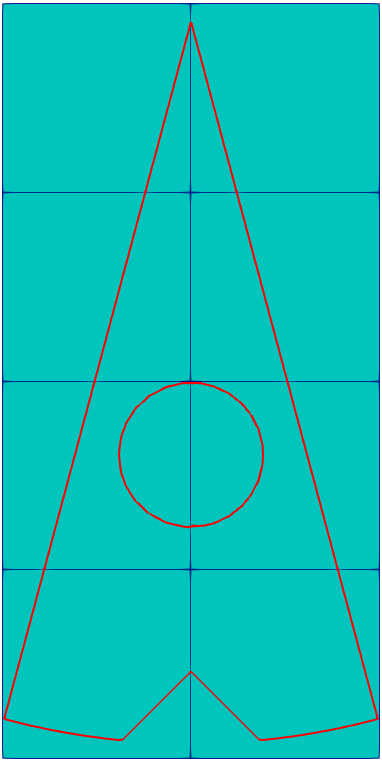
\includegraphics[width=0.14\textwidth]{pie_refined1.png}
  \label{f:pieref1}
 }
\centering
 \subfigure[~]{
  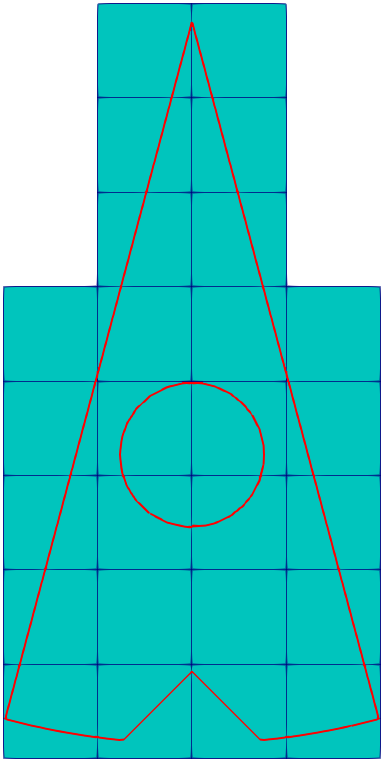
\includegraphics[width=0.14\textwidth]{pie_refined2.png}
  \label{f:pieref2}
 }
\centering
 \subfigure[~]{
  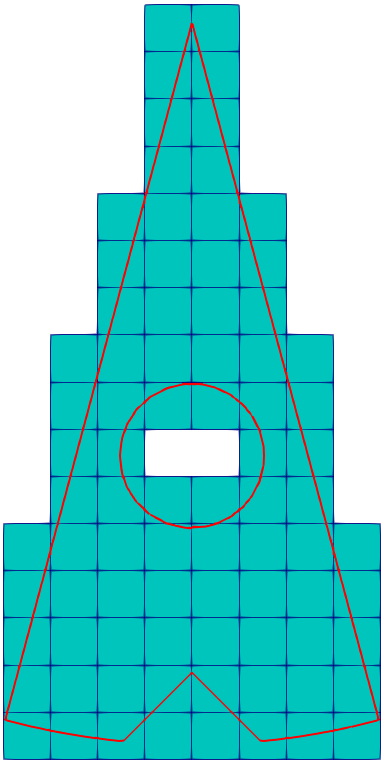
\includegraphics[width=0.14\textwidth]{pie_refined3.png}
  \label{f:pieref3}
 }
\centering
 \subfigure[~]{
  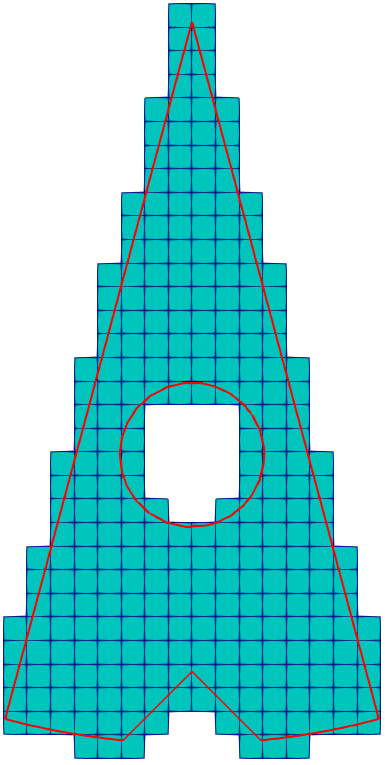
\includegraphics[width=0.14\textwidth]{pie_refined4.png}
  \label{f:pieref4}
 }
\centering
 \subfigure[~]{
  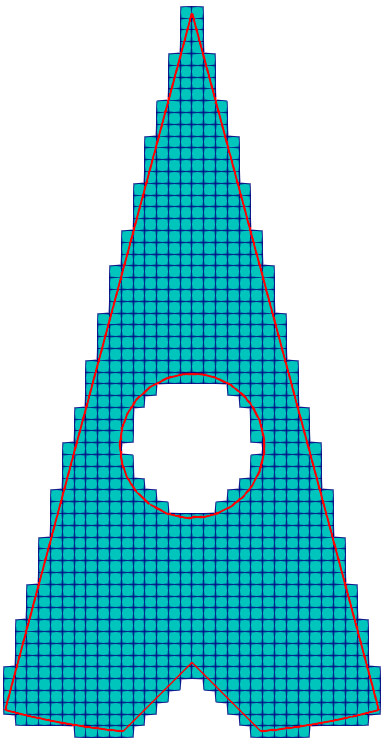
\includegraphics[width=0.14\textwidth]{pie_refined5.png}
  \label{f:pieref5}
 }
\centering
 \subfigure[~]{
  
\includegraphics[width=0.14\textwidth]{pie_refined6.png}
  \label{f:pieref6}
 }
 \caption{Effect of the refinement level applied on the complete structure (\texttt{-a} switch), (1 to 6)}
\label{fig:pieref}
\end{figure}


\begin{figure}[htb]
\centering
 \subfigure[~]{
  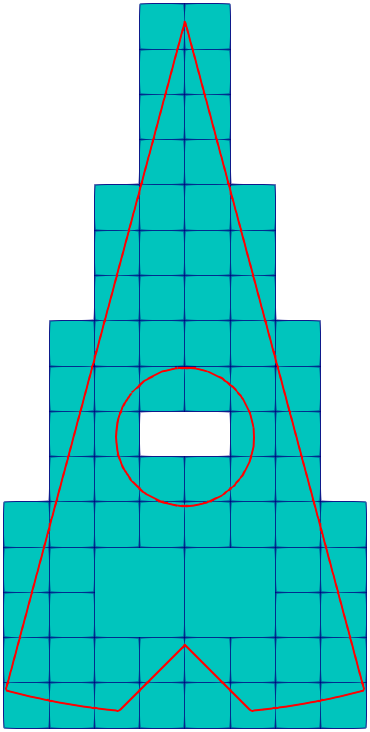
\includegraphics[width=0.22\textwidth]{pie_refined2s3.png}
  \label{f:pierefs3}
 }
\centering
 \subfigure[~]{
  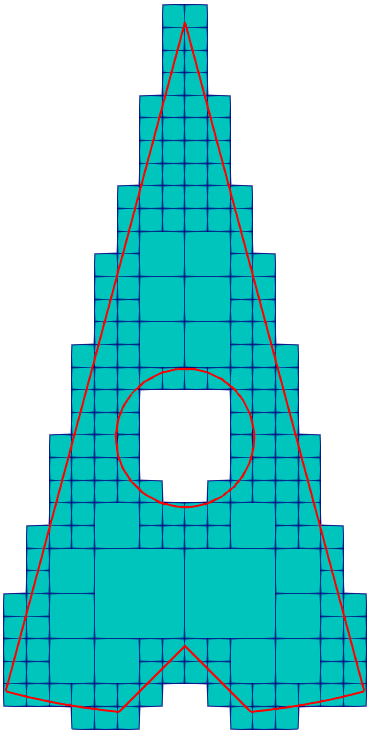
\includegraphics[width=0.22\textwidth]{pie_refined2s4.png}
  \label{f:pierefs4}
 }
\centering
 \subfigure[~]{
  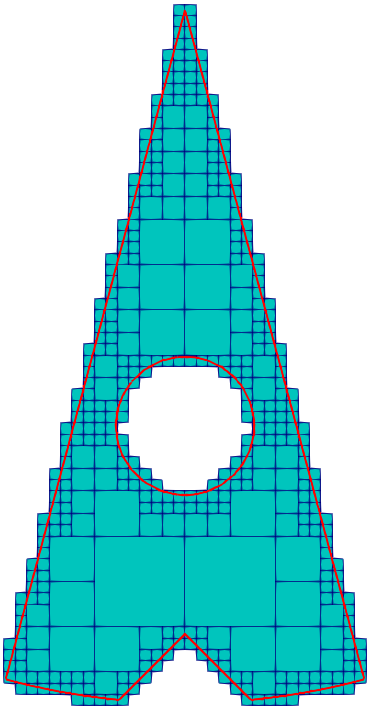
\includegraphics[width=0.22\textwidth]{pie_refined2s5.png}
  \label{f:pierefs5}
 }
\centering
 \subfigure[~]{
  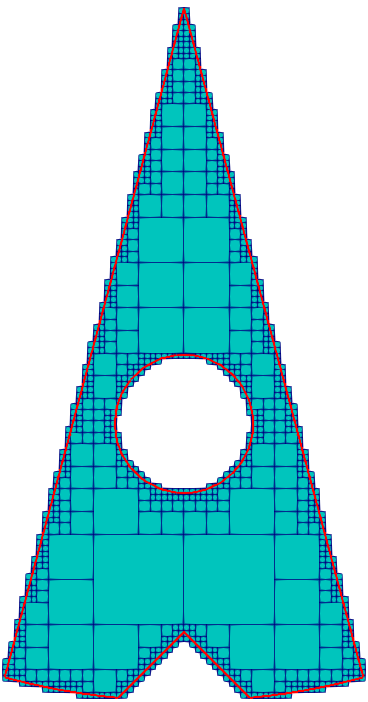
\includegraphics[width=0.22\textwidth]{pie_refined2s6.png}
  \label{f:pierefs6}
 }
 \caption{Effect of combined refinement levels, with level 2 applied on the complete structure (\texttt{-a} switch), and incremental refinement (3 to 6) only applied on surface quadrants (\texttt{-s} switch).}
\label{fig:pierefs}
\end{figure}


\begin{figure}[htb]
\centering
 \subfigure[~]{
  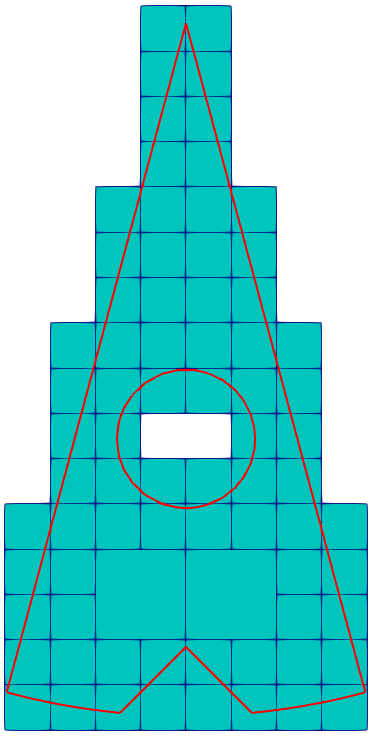
\includegraphics[width=0.22\textwidth]{pie_balanced2s3.png}
  \label{f:piebals3}
 }
\centering
 \subfigure[~]{
  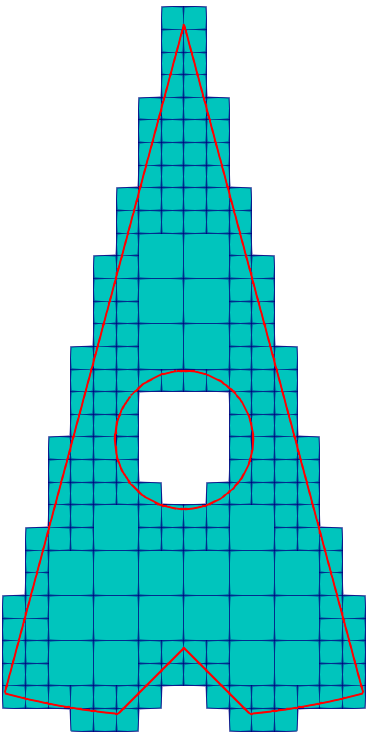
\includegraphics[width=0.22\textwidth]{pie_balanced2s4.png}
  \label{f:piebals4}
 }
\centering
 \subfigure[~]{
  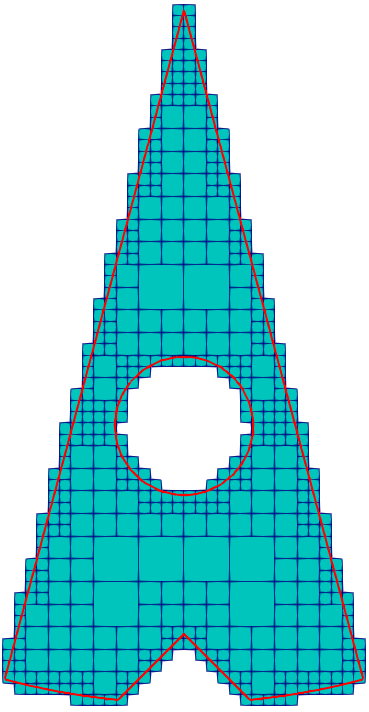
\includegraphics[width=0.22\textwidth]{pie_balanced2s5.png}
  \label{f:piebals5}
 }
\centering
 \subfigure[~]{
  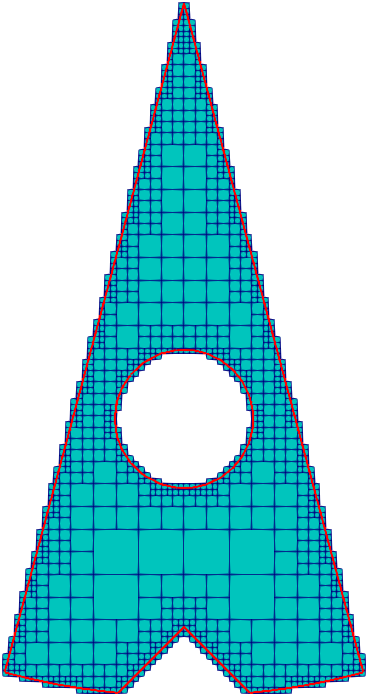
\includegraphics[width=0.22\textwidth]{pie_balanced2s6.png}
  \label{f:piebals6}
 }
 \caption{After the balancing step, note that in the first case, nothing is to be done.}
\label{fig:pielabs}
\end{figure}


\begin{figure}[htb]
\centering
 \subfigure[~]{
  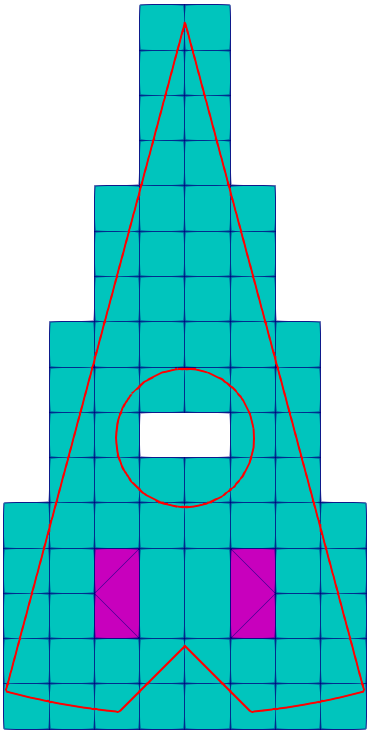
\includegraphics[width=0.22\textwidth]{pie_transition2s3.png}
  \label{f:pietranss3}
 }
\centering
 \subfigure[~]{
  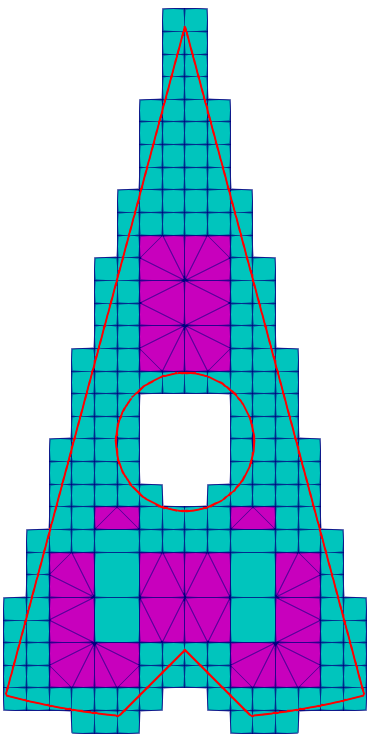
\includegraphics[width=0.22\textwidth]{pie_transition2s4.png}
  \label{f:pietranss4}
 }
\centering
 \subfigure[~]{
  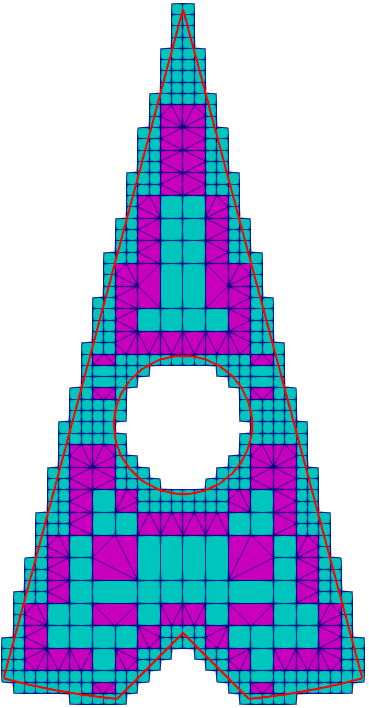
\includegraphics[width=0.22\textwidth]{pie_transition2s5.png}
  \label{f:pietranss5}
 }
\centering
 \subfigure[~]{
  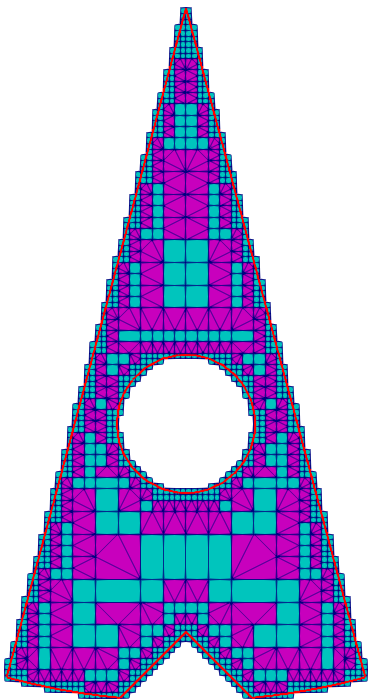
\includegraphics[width=0.22\textwidth]{pie_transition2s6.png}
  \label{f:pietranss6}
 }
 \caption{After the transition step. Note that the more difference between levels, the more transition patterns are used\ldots}
\label{fig:pielabs}
\end{figure}

%---------------------------
%---------------------------
\section{Fitting quadrants to Input Surface}
\label{sec:method}
%---------------------------
%---------------------------



\begin{algorithm}[H]

\SetAlgoLined
\KwResult{A mixed-elements mesh}
 \tcc{Preprocess: handle boundary}
 \tcc{Generate quadtree}
\nl \ForEach{Quadrant}{
 \Repeat {desired Refinement Level}{
 \nl Subdivide Quadrant\;
   \ForEach{ new Sub-Quadrant}{
   \If{Intersects Input \textit{or} Is Inside}{Insert Sub-Quadrant}
    }
  }\label{alg:subdivide}
  }
 \nl Create balanced quadtree\; \label{alg:goto}
 \nl Apply Transition Patterns\;
 \tcc{Input surface fitting}
 \nl Detect Features in Input\;
 Project Close to Boundary\;
 Remove on Input Surface\;
 Shrink to Boundary\;
 \nl Apply Surface Patterns\;
 \caption{Generation process and Input surface fitting}
 \label{alg:surfacefitting}
\end{algorithm}

%---------------------------
\subsection{Boundary and sharp features handling}

preprocess

 \begin{figure}[htb]
\centering
 \subfigure[~]{
  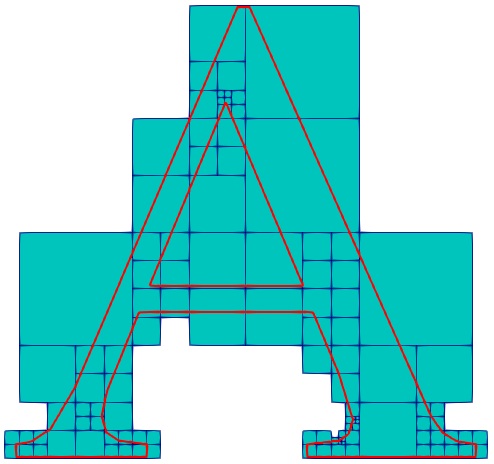
\includegraphics[width=0.3\textwidth]{a_boundary.png}
  \label{f:boundary}
 }
\caption{After boundary handling.}
\label{fig:boundary}
\end{figure}

The first step to 

        // test1: if nb Features >= 2
        // first condition is optimization if NbFeatures has been already computed
        // test2: if distFProjectionFeature > distMax for each node
        // done: compute distMax before...
        // test3: if the number of intersection of the Polyline and Quadrant edge >= 3


%---------------------------
\subsection{Generating first quadrants over boundary prepared mesh}


\begin{figure}[htb]
\centering
 \subfigure[~]{
  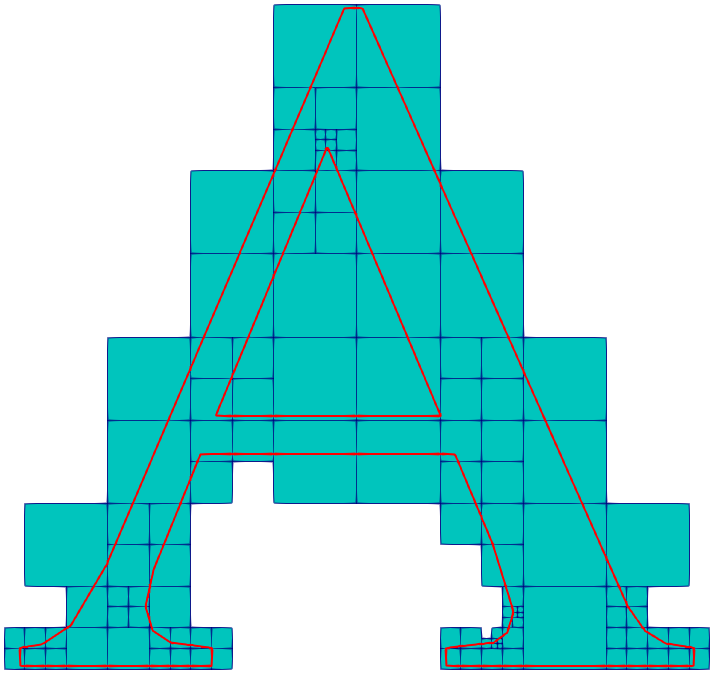
\includegraphics[width=0.3\textwidth]{a3_boundary_refined.png}
  \label{f:boundaryref3}
 }
  \subfigure[~]{
  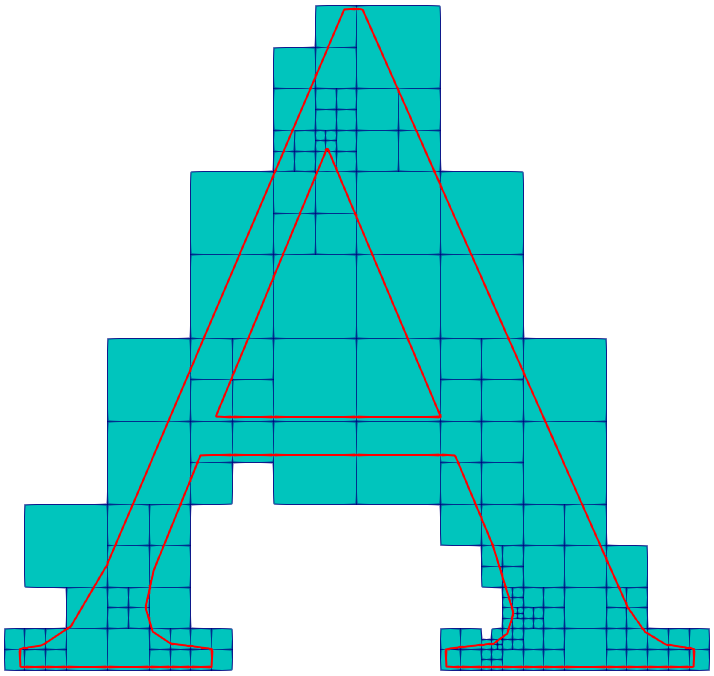
\includegraphics[width=0.3\textwidth]{a3_boundary_balanced.png}
  \label{f:boundarybal3}
 }
 \subfigure[~]{
  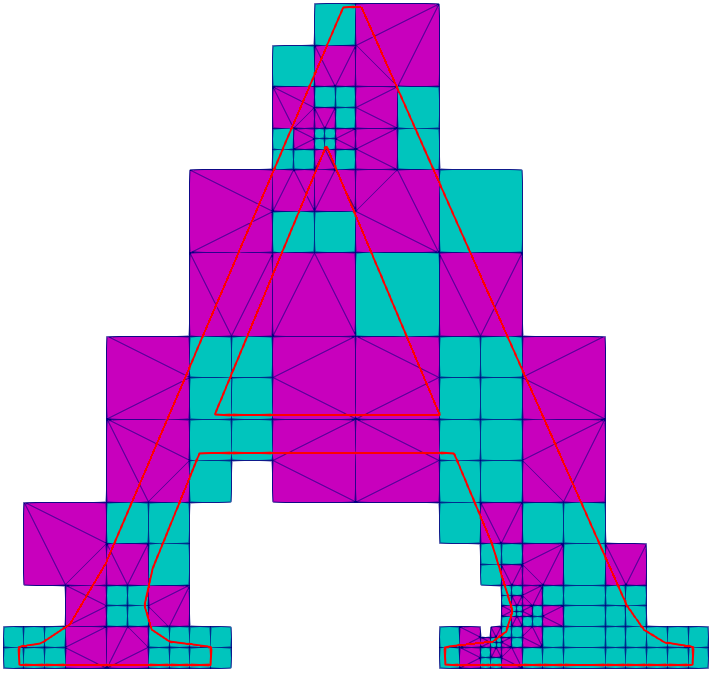
\includegraphics[width=0.3\textwidth]{a3_boundary_transition.png}
  \label{f:boundarytrans3}
 }
 \caption{After refinement, balancing and transition steps, level 3.}
\label{fig:generate3}
\end{figure}

\begin{figure}[htb]
\centering
 \subfigure[~]{
  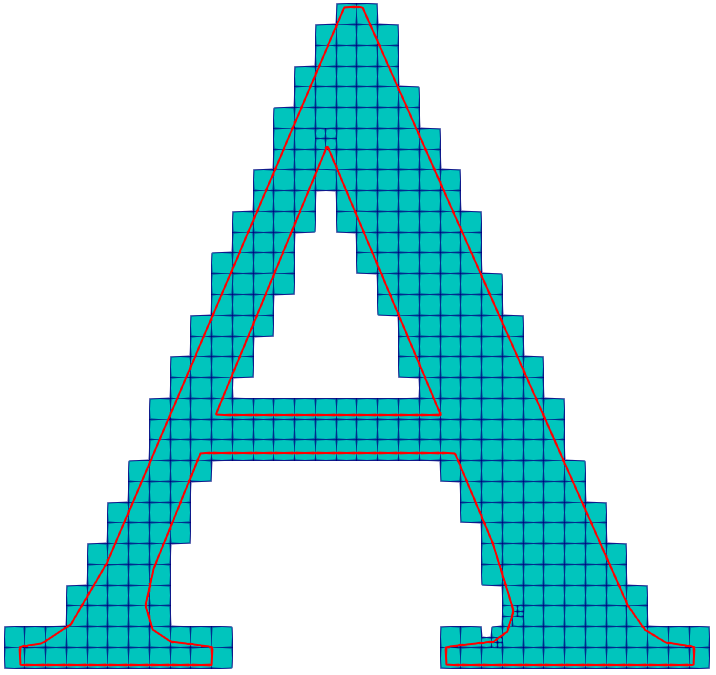
\includegraphics[width=0.3\textwidth]{a5_boundary_refined.png}
  \label{f:boundaryref5}
 }
  \subfigure[~]{
  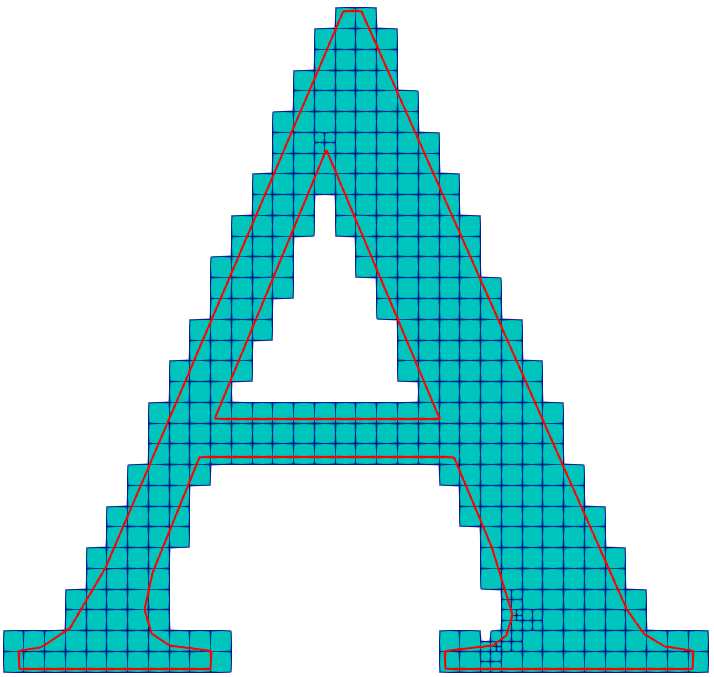
\includegraphics[width=0.3\textwidth]{a5_boundary_balanced.png}
  \label{f:boundarybal5}
 }
 \subfigure[~]{
  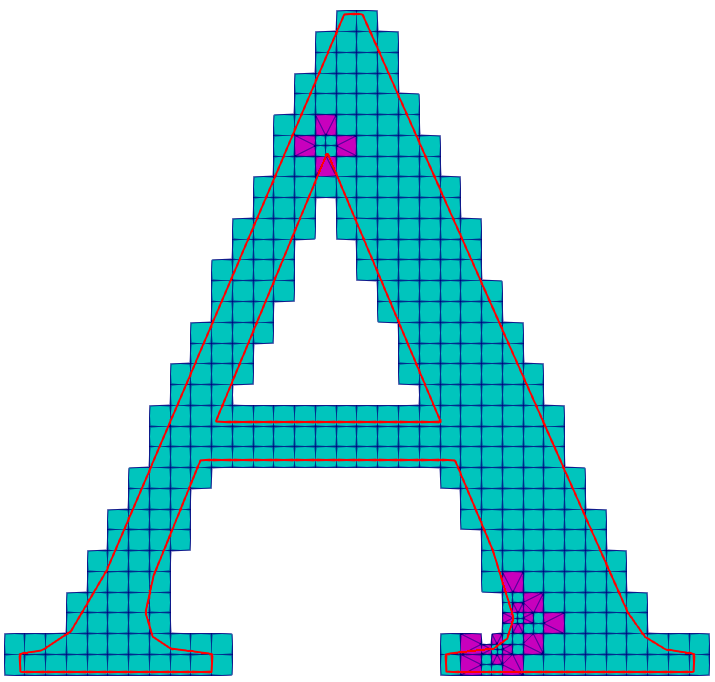
\includegraphics[width=0.3\textwidth]{a5_boundary_transition.png}
  \label{f:boundarytrans5}
 }
 \caption{After refinement, balancing and transition steps, level 5.}
\label{fig:generate5}
\end{figure}

\begin{figure}[htb]
\centering
 \subfigure[~]{
  
\includegraphics[width=0.3\textwidth]{a7_boundary_refined.png}
  \label{f:boundaryref7}
 }
  \subfigure[~]{
  
\includegraphics[width=0.3\textwidth]{a7_boundary_balanced.png}
  \label{f:boundarybal7}
 }
 \subfigure[~]{
  
\includegraphics[width=0.3\textwidth]{a7_boundary_transition.png}
  \label{f:boundarytrans7}
 }
 \caption{After refinement, balancing and transition steps, level 7.}
\label{fig:generate7}
\end{figure}


%---------------------------
\subsection{Handling Input surface}

\begin{figure}[htb]
\centering
 \subfigure[~]{
  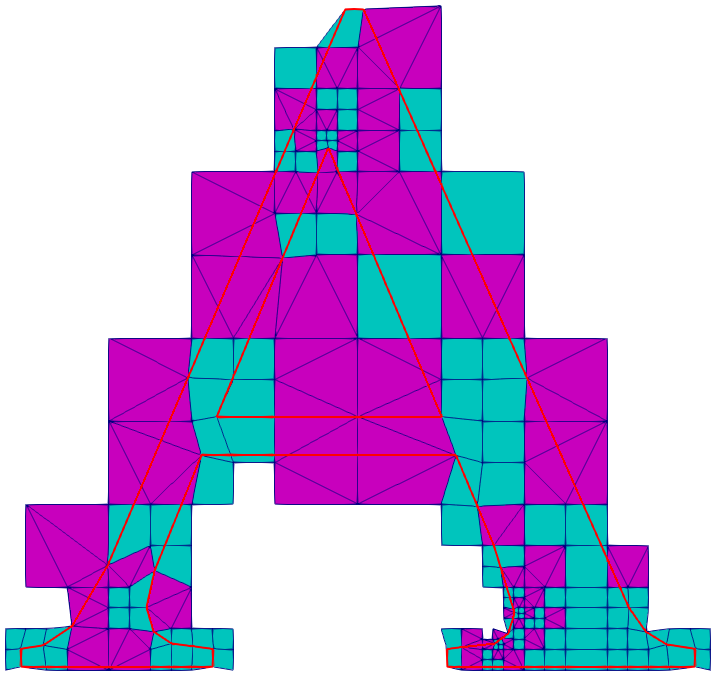
\includegraphics[width=0.3\textwidth]{a3_boundary_projectinteriorcloseto.png}
  \label{f:boundaryclose3}
 }
 \subfigure[~]{
  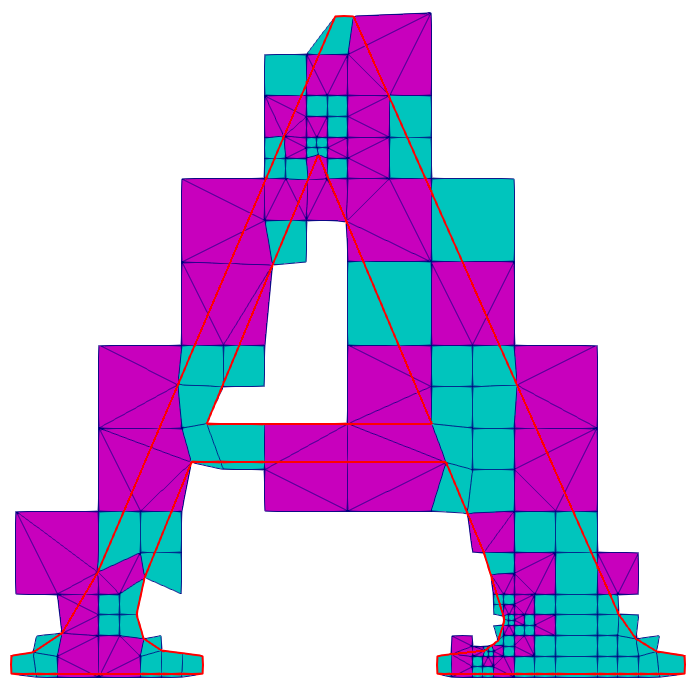
\includegraphics[width=0.3\textwidth]{a3_boundary_removesurface.png}
  \label{f:boundaryrem3}
 }\\
  \subfigure[~]{
  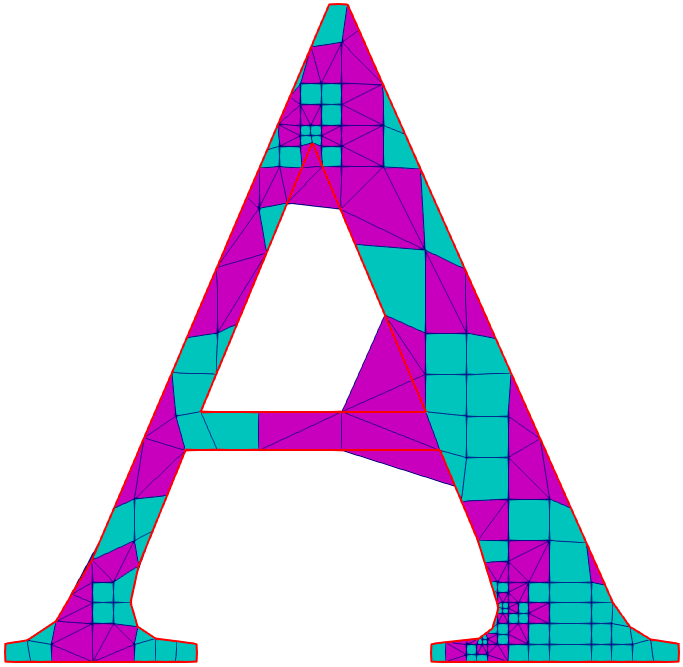
\includegraphics[width=0.3\textwidth]{a3_boundary_shrinkexterior.png}
  \label{f:boundaryshrink3}
 }
  \subfigure[~]{
  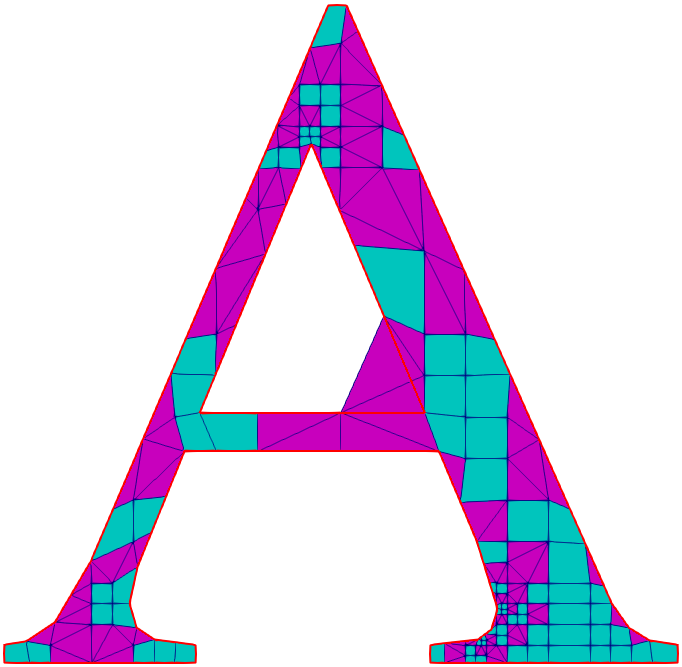
\includegraphics[width=0.3\textwidth]{a3_boundary_surfacepatterns.png}
  \label{f:boundarysurf3}
 }
 \caption{After projecting interior points close to boundary, , level 3.}
\label{fig:surfacehandling3}
\end{figure}
%
\begin{figure}[htb]
\centering
 \subfigure[~]{
  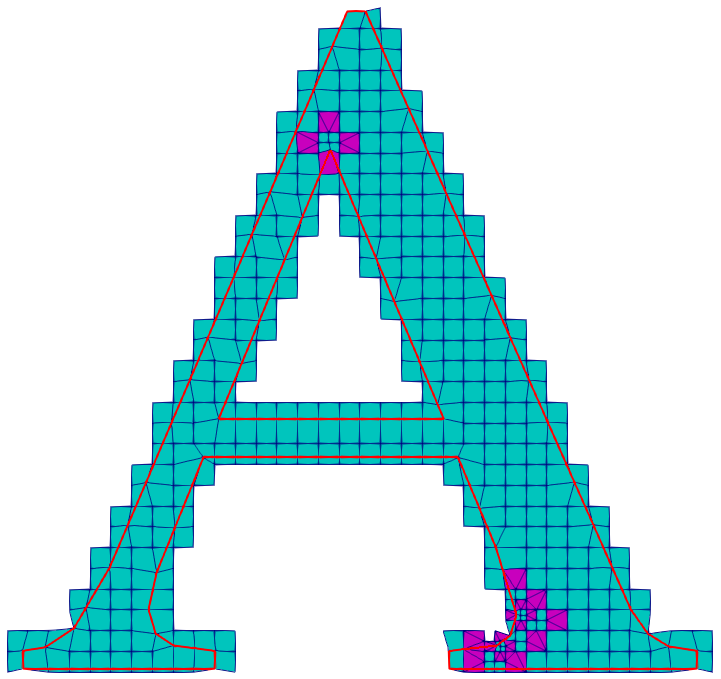
\includegraphics[width=0.3\textwidth]{a5_boundary_projectinteriorcloseto.png}
  \label{f:boundaryclose5}
 }
 \subfigure[~]{
  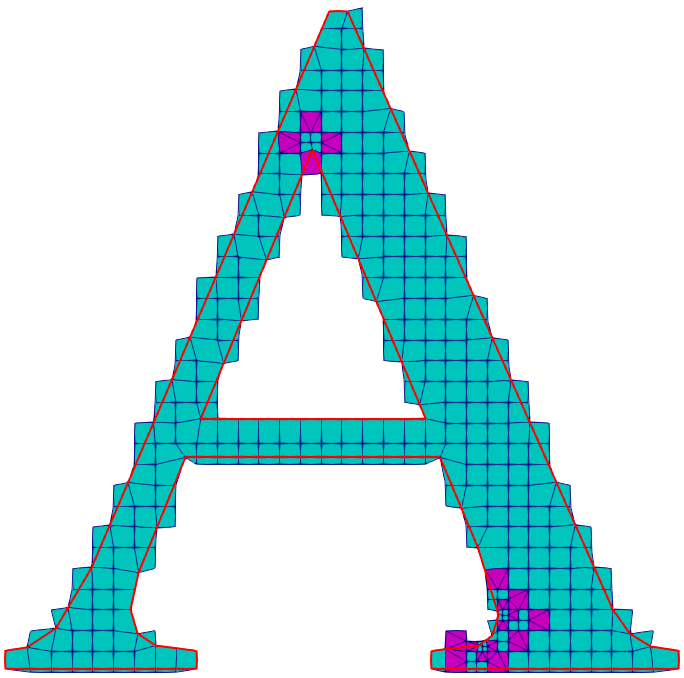
\includegraphics[width=0.3\textwidth]{a5_boundary_removesurface.png}
  \label{f:boundaryrem5}
 }
 \\
  \subfigure[~]{
  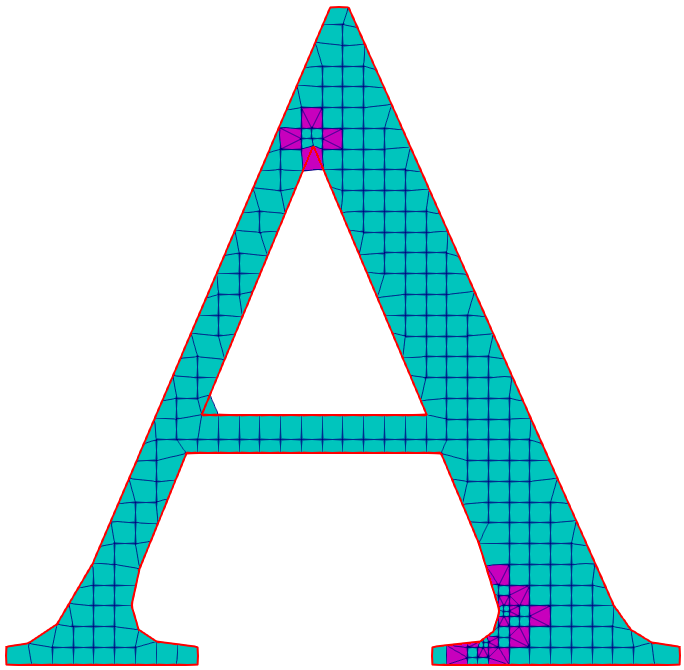
\includegraphics[width=0.3\textwidth]{a5_boundary_shrinkexterior.png}
  \label{f:boundaryshrink5}
 }
  \subfigure[~]{
  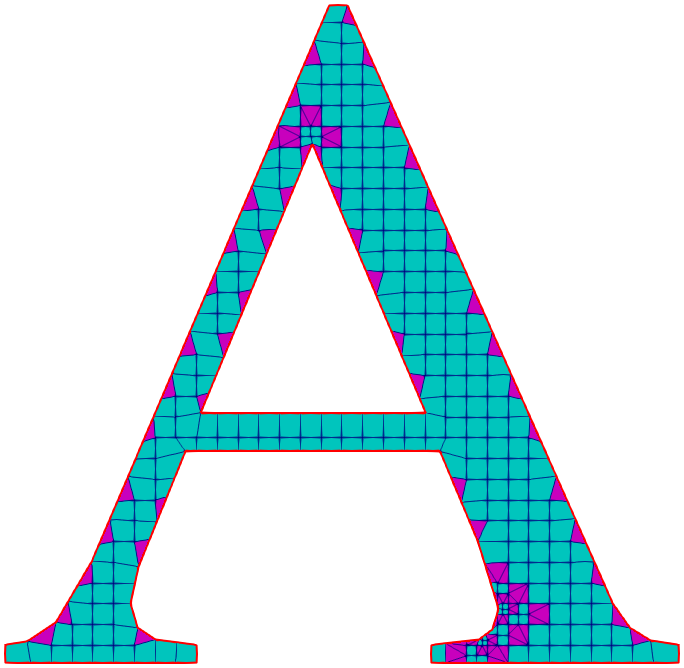
\includegraphics[width=0.3\textwidth]{a5_boundary_surfacepatterns.png}
  \label{f:boundarysurf5}
 }
 \caption{After projecting interior points close to boundary, level 5.}
\label{fig:surfacehandling5}
\end{figure}
%
\begin{figure}[htb]
\centering
 \subfigure[~]{
  
\includegraphics[width=0.3\textwidth]{a7_boundary_projectinteriorcloseto.png}
  \label{f:boundaryclose7}
 }
 \subfigure[~]{
  
\includegraphics[width=0.3\textwidth]{a7_boundary_removesurface.png}
  \label{f:boundaryrem7}
 }\\
  \subfigure[~]{
  
\includegraphics[width=0.3\textwidth]{a7_boundary_shrinkexterior.png}
  \label{f:boundaryshrink7}
 }
  \subfigure[~]{
  
\includegraphics[width=0.3\textwidth]{a7_boundary_surfacepatterns.png}
  \label{f:boundarysurf7}
 }
 \caption{After projecting interior points close to boundary, level 7.}
\label{fig:surfacehandling7}
\end{figure}



%---------------------------
%---------------------------
\section{Remeshing}
\label{sec:remeshing}
%---------------------------
%---------------------------


\begin{algorithm}[H]
\SetAlgoLined
\SetKw{kwGoto}{Goto}
\KwResult{A refined mixed-elements mesh}
 \ForEach{Element to refine}{
  Identify containing Quadrant\;
  Subdivide Quadrant\;
   \ForEach{Sub-quadrant}{
   \If{Intersect input \textit{or} Is In}{Insert Sub-Quadrant}
    }
  }
  \kwGoto{Algorithm \ref{alg:generate}, step \ref{alg:goto}}
 \caption{Refinement process}
\end{algorithm}

identify which Quad contains the element, information from file

subdivide Quad + goto subsection balanced

(local remeshing? neighbourhood??)


%---------------------------
%---------------------------
\section{Installing}
\label{install}
%---------------------------
%---------------------------

In order to install this application you will need a Unix--based system, a \texttt{c++} compiler and \texttt{cmake}. You should do the following:

%---------------------------
\subsection{Create an account on github.com}

\begin{itemize}
\item go to github.com, then 'Signup and Pricing' $\Rightarrow$ 'Free for open source' $\Rightarrow$ 'Create a free account'
\item choose Username/Email/Password and it's done
\item you can also update your account settings (website, avatar...)
\end {itemize}

%---------------------------
\subsection{Git Fork MixedQuadTree}

Let's fork the initial MEPP repository. So, once you're logged in on github
\begin{itemize}
\item go to https://github.com/jaillet/MixedQuadTree/
\item click on the 'Fork' button
\item once the fork is finished, you'll have your own copy of MixedQuadTree with the following path: https://github.com/\textbf{yourUsername}/MixedQuadTree
\item at this URL, you're able to browse the sources, see the commit log, report issues...
\end {itemize}

%---------------------------
\subsection{Compiling}

{\small
\begin{verbatim}
$ git clone /https://github.com/jaillet/MixedQuadTree.git
$ cd MixedQuadTree/
$ git checkout branch develop
$ mkdir build ; cd build
$ cmake ../src -D_CMAKE_BUILD_TYPE=Debug (or Release) // Uppercase is important
$ cmake .
$ make -j#nproc
\end{verbatim}
}

This has been tested on Linux and Mac without any known error nor warning.

\subsection{Git usage}
At this point, you can edit and commit files using  the git workflow 
 
\textbf{but only push to your own fork of MixedQuadTree (origin) !!!}\\

The merge between the original repository is done by ANOTHER DEVELOPER after a \textbf{'pull request'}.
To make a 'pull request', go to https://github.com/yourUsername/MixedQuadTree, click on 'Pull Request'. Then, choose the two branches you would like to merge (master in \textit{jaillet} and yourbranch in origin), write your comments and click on 'Send Pull Request'.

%%---------------------------
%%---------------------------
%\section{Standalone program use}
%\label{standalone}
%%---------------------------
%%---------------------------
%
%
%This mesh generator will allow you to create a mixed--element mesh starting from a surface mesh composed of triangles. Let this input surface mesh be $\mathcal{S}$. Two constraints must be fulfilled by $\mathcal{S}$: it must be unfolded (no self--intersection), and the normal of the triangles must be pointing outside.
%
%The algorithm will use $\mathcal{S}$ for two purposes: to find out if a point is inside or outside the domain and to project a point onto $\mathcal{S}$. Therefore, if you have two different meshes representing the exact same domain, you should use the one with less triangles. The algorithm will compute faster the output volume mesh.
%
%The first step of the algorithm is to compute the Bounding box (Bbox) of $\mathcal{S}$. This Bbox will not necessarily be a perfect hexahedron (cube). Therefore, an algorithm will be employed to automatically compute a set of cubes containing $\mathcal{S}$. For instance, if $\mathcal{S}$ is a baseball bat, the starting point will be 3 or 4 cubes, one  next to the other.
%
%Now it is possible to introduce the other important input: the Refinement Level (\textit{rl}). This mesh generator is based on the  Octree technique \cite{Yerry1984,Shephard1991}. This technique recursively split an Octant in a finite number of equivalent sons. For instance if the Octant is a cube, to refine it one level means that it will be replaced by 8 new Octants. All of them will be sons of the replaced Octant in the Octree structure. Note that in some works this splitting operation produces 27 new cubes each time an Octant is refined \cite{Schneiders1996,Zhang2006,Ito2009}. In our case, Octants will continue to refine until a maximum provided level is reached. Octants lying completely outside $\mathcal{S}$ will be removed.
%
%To produce a mesh you must execute in a terminal the following:
%
%{\small
%\begin{verbatim}
%$ ./mesher_roi [-option | parameters]
%\end{verbatim}
%}
%
%%---------------------------
%%---------------------------
%\subsection{Basic mesh generation}
%\label{generatemesh}
%%---------------------------
%%---------------------------
%
%If you do not indicate any option nor parameters, the program will list all the available options for you. The basic mesh generation options are listed below. It is mandatory to provide a surface triangular mesh that describes the domain to mesh. Basic input/output formats are the following:
%
%\begin{itemize}
%\item \texttt{-d}: next to it comes the name of an input file (\texttt{mdl} extension) where the surface mesh is specified. In this version of the code only one input surface can be specified.
%\item \texttt{-o}: another option to specify an input: \texttt{off} format file.
%\item \texttt{-u}: next to it comes the name of the output file. The extension (file format) will be automatically added: \texttt{mvm} (Mixed Volumen Mesh) is by default, but it can be changed with the next two options.
%\item \texttt{-g}: save the ouput mesh in \textsc{GetFem} format: \texttt{gmf} extenstion (Getfem Mesh Format). Note you can still specify an output file name with option \texttt{-u}, \textit{e.g.}: \texttt{-u myoutput -g} will produce output file: \texttt{myoutput.gmf}.
%\item \texttt{-v}: equivalent to option \texttt{-g}, but saves in \textsc{vtk -- ascii} format.
%\end{itemize}
%
%Now, to provide the Refinement Level (\textit{rl}) several options can be used:
%
%\begin{itemize}
%\item \texttt{-a}: next to it comes the number of times ($N$) the splitting operation will be performed over the initial octants enclosing $\mathcal{S}$. For instance if we type: \texttt{-a 2} this will split all the intial octants into eight new ones and each one of them in eight more.
%\item \texttt{-s}: next to it comes the number of times ($N$) the splitting operation will be performed over each octant that intersects a section of $\mathcal{S}$. For instance if we type: \texttt{-s 2} this will split all the intial octants into eight new ones and  then, only the octants that still intersect $\mathcal{S}$ will be split in eight more.
%\item \texttt{-b}: next to it comes the name of file where some block regions are specified. A block is defined by 2 points: $(min_x, min_y, min_z), ((max_x, max_y, max_z)$ and a \textit{rl} to be applyed over the octants that intersect this block. This is a text file where first we specify the number of blocks and then we detail each one of them. An example with 2 regions is now provided:
%
%\begin{minipage}{0.2\textwidth}
%\begin{verbatim}
%n_regions 2
%
%0 0 0
%10 10 10
%5
%
%0 0 0
%20 20 20
%4
%\end{verbatim}
%\end{minipage}
%\hfill
%\begin{minipage}[c]{0.65\textwidth}
%In this case the portion of $\mathcal{S}$ intersecting the hexahedron $(0,0,0) \to (10,10,10)$ will be refined to level 5 and the complement inside the block $(0,0,0) \to (20,20,20)$ that intersects $\mathcal{S}$ will be refined to level 4.\\[0.2cm]
%
%\textbf{Important Note}: if an octant belongs within more than one refinement region (no matter the type of it), it will be refined to maximum level among those regions.
%\end{minipage}
%\item \texttt{-r}: next to it comes 2 arguments; the name of file where another input surface is specified in \texttt{mdl} format and a \textit{rl}. All the octants inside $\mathcal{S}$ and the specified region will be refined to \textit{rl}. Note that this geometry can be any closed triangle mesh, for instance a tetrahedron. Also note that mesh generation time will be directly influenced by the number of triangle faces the input meshes have. In order to accelerate the process you should use as less triangles as possible that correctly define the input domains and regions. Let us say that the mesh called \texttt{myregion.mdl} intersects a portion of $\mathcal{S}$, then the instruction: \texttt{-r myregion.mdl 5} will refine to level 5 all the octants in that region. The last point regarding this option is automatic rotation. The code will compute the ``dominant normals'' of the input region and will try to align them with referential axes. This transformation will also be applied to $\mathcal{S}$. Once the mesh is generated, the inverse transformation will be applied to the output so the domain is well represented.
%\end{itemize}
%
%Finally, note that ``big'' meshes can be produced with a small value for $N$. For instance, if the starting point is only one cube and we set $N=9$, the code may produce up to $8^9 = 134,217,728$ elements.
%
%Let illustrate all this with the followig example: \texttt{./mesher\_roi -o cortex.off -r reg.mdl 5 -s 5 -u out -g}. Meaning that $\mathcal{S}$ is defined in input file \texttt{cortex.off} in \texttt{off} format, then another surface that intersects a portion of $\mathcal{S}$ is defined in file \texttt{reg.mdl} and the octants in that region must be refined to level 5. At the same time, every octant intersecting the surface must also be refined to level 5 and all the rest are as big as possible. Finally output must be written to file \texttt{out.gmf} in \textsc{GetFem} mesh format. The inputs and outputs of this execution can be seen in Figure \ref{f:mesheroi}.
%
% \begin{figure}[htb]
%\centering
% \subfigure[~]{
%  
\includegraphics[width=0.28\textwidth]{a_polyline.png}
%  \label{f:roic}
% }
% \subfigure[~]{
%  
\includegraphics[width=0.26\textwidth]{a_polyline.png}
%  \label{f:roicsurf}
% }
% \subfigure[~]{
%  
\includegraphics[width=0.24\textwidth]{a_polyline.png}
%  \label{f:roiccut}
% }
%\caption{An example with different refinement levels: \subref{f:roic} input surface mesh and region of refinement specified by another surface mesh, \subref{f:roicsurf} the surface of the output mesh and \subref{f:roiccut} the same output with a saggital cut where the alignement with the region of refinement in the top front section of the brain is perfect.}
%\label{f:mesheroi}
%\end{figure}
%
%%---------------------------
%%---------------------------
%\subsection{Advanced mesh generation}
%\label{regeneratemesh}
%%---------------------------
%%---------------------------
%
%When generating a mesh with the code explained in section \ref{generatemesh}, an octant mesh file will be automatically written. Using the octant file (extension .oct) elements, octants and even regions of the generated mesh can be refined. Actually, only octants can be subdivided in 8 new octants (cubes), however, if a particular element must be refined the octant file allows to detect to which octant it belongs and refine it. All the refinement options of setcion \ref{generatemesh} can be used and one extra option to list particular elements of the mesh can be employed.
%
%Following the example of setcion \ref{generatemesh}, we can now execute: \texttt{./mesher\_roi -d cortex.mdl -c out.oct -a 4 -l list.txt -u test -v} generating the result shown in Figure \ref{f:mesheroi2}.
%
% \begin{figure}[htb]
% \centering
%  
\includegraphics[width=0.28\textwidth]{a_polyline.png}
%\caption{An example starting from a previous generated mesh. Section inside the red circle are a list of elements we want to refine only once.}
%\label{f:mesheroi2}
%\end{figure}
%
%As you noticed, in this example we start from octant mesh already generated \texttt{out.oct}, so the element alignement is conserved as in previous example. We then specify that all the octants in the mesh must, at least, count with a refinement level 4 (\texttt{-a 4}). Then we can provide a simple text file listing specific element index we want to refine. One element per line and that is all (no element count needed). Please note that is plain text file only (be shure not to be using rtf files which add more information). In the example these elements are placed in bottom back portion of the brain inside a red circle. All the elements will be refined exactly one extra time, therefor it is not necessary to specify a target refinement level. Finally this will generate two outputs: \texttt{test.vtk} and \texttt{test.oct}. The first is because we specified option \texttt{-v} and the last because we will always generate and oct file in case further refinement is required. 
%
%\textbf{Note}: even if it is possible to generate elements of different refinement level at boundary of the domain, it is not recommended because most of the times this leads to invalid (inverted) elements. In the previous example, as next to boundary octants were refined one extra level (to level 6) it would be safer to have also refined the entire surface to level 6 (with option \texttt{-s 6}).
%
%%---------------------------
%%---------------------------
%\section{Using the code from another program}
%\label{inside}
%%---------------------------
%%---------------------------
%
%In order to generate a volume mesh, we only need a list of nodes, a list of triangular faces and the refinement level. This section explains how to interact with the code if you want to program your own application. For example, this is useful if you have a surface mesh that is not in the proper file format, or you need to write the output in another file format.
%
%File \texttt{Main.cpp} is in charge of input reading, executing the mesh generator with proper parameters and write the output. In order to specify an input surface mesh, we need to create a \texttt{TriMesh} object. This object is composed of two vectors: one with the points and the other with triangles. The Points are specified through instances of class Point3D as follow:
%
%{\small
%\begin{verbatim}
%1. vector<Point3D> points; //the vector of points
%2. points.reserve(1);      //re-size the vector if you know the quantity of nodes
%3. double x=0, y=0, z=0;   //define the coordinates of a point
%4. Point3D p(x,y,z);       //create a point
%5. points.push_back(p);   //add the point to the vector
%\end{verbatim}
%}
%
%Now for the faces and create a surface mesh: \texttt{TriMesh} object with both vectors (points and faces).
%
%{\small
%\begin{verbatim}
%1. vector<vector<unsigned int> > faces; //the vector of faces
%2. faces.reserve(1);                    //re-size the vector
%3. vector<unsigned int> a_face(3,0);    //define a face with 3 nodes
%4. a_face[1] = 1; a_face[2] = 2;        //update references
%5. faces.push_back(a_face);             //add the point to the vector
%6. TriMesh tm1(points,faces); //create a surface mesh
%\end{verbatim}
%}
%
%Provide the maximum refinement level among all the options requiered to generate the output mesh. This value enables important optimization in time.
%
%{\small
%\begin{verbatim}
%1. list<RefinementRegion *> all_regions;
%2. RefinementRegion *rr = new RefinementAllRegion(4);
%3. all_regions.push_back(rr);
%4. Mesher mesher;   
%5. unsigned int max_ref_level = 4;
%6. FEMesh output = mesher.generateMesh(tm1,ref_level,out_name,all_regions);
%7. vector<Point3D> output_pts = output.getPoints();
%8. vector<vector<unsigned int> > output_elem = output.getElements();
%9. cout <<''X: ''<<output_pts[0][0]<<'' Y: ''<<output_pts[0][1]<<''X: ''<<output_pts[0][2]<<'\n'; 
%\end{verbatim}
%}
%
%Now you can handle the points of the output mesh as shown at line 9 of the previous code: \texttt{output\_pts[n]} will give you access to point \texttt{n} and then you can access its coordinates with another vector accesss. For instance, coordinate \texttt{z} of point \texttt{n} is at \texttt{output\_pts[n][2]}. As for the elements, they are in the vector. Each component of  the vector is a new element where the index of the nodes defining the element are in another vector. For instance the second node of the first element is at \texttt{output\_elem[0][1]}. The notation (order of the nodes index) for each type of element is defined in section \ref{conventions}.
%
%Please see class \texttt{Main.cpp} in the source files to known how to define the other types of regions.
%
%%---------------------------
%%---------------------------
%\section{Element node conventions and mvm extension}
%\label{conventions}
%%---------------------------
%%---------------------------
%
%The Mixed Volume Mesh format allows to easily describe a mesh composed of different element types. It will be extended later, but for the moment it can manage the four basic element types generated by the meshing technique. 
%
%\begin{minipage}{0.2\textwidth}
%\begin{verbatim}
%MIXED
%6 2
%
%-1  1 -1
%-1  1  1
% 1  1  1
% 1  1 -1
% 0  3  0
% 3  1  0
%
%P 0 1 2 3 4
%T 2 3 4 5
%\end{verbatim}
%\vspace{.3cm}
%\end{minipage}
%\hfill
%\begin{minipage}[c]{0.78\textwidth}
%This example of the \texttt{mvm} format shows the syntax. First goes the header ``MIXED'', then the number of nodes and the number of elements in the mesh. After that there is the list of coordinates X, Y and Z for each node. The first node has index 0 and so on until the last one. In the example the last node has index 5. Finally there is the list of elements. The description of an element starts with a string. The four basic employs: \texttt{H} for the hexahedron, \texttt{R} for the prism, \texttt{P} for the pyramid and \texttt{T} for the tetrahedron. 
%
%\textbf{Important Note}: some elements employ more than one character to specify its type. For instance, \texttt{P6} corresponds to a pentagonal base pyramid (having in total 6 nodes).
%\end{minipage}
%
%The four basic element types considered in this work are shown in Figure \ref{elementsNumbering}. For instance if we define a prism (wedge) with the following indexes: 11 20 19 0 8 4, it means that one triangular face $t$, is defined by indexes: 11, 20 and 19. Moreover, nodes 0, 8 and 4 will have a positive distance w.r.t. to $t$, when its normal is computed  counterclockwise. 
% 
% \begin{figure}[htb]
%\centering
% \subfigure[~]{
%  
\includegraphics[width=0.18\textwidth]{a_polyline.png}
%  \label{f:basic_hex}
% }
% \subfigure[~]{
%  
\includegraphics[width=0.18\textwidth]{a_polyline.png}
%  \label{f:basic_prism}
% }
% \subfigure[~]{
%  \includegraphics[width=0.18\textwidth]{a_polyline.png}
%  \label{f:basic_pyramid}
% }
% \subfigure[~]{
%  \includegraphics[width=0.18\textwidth]{a_polyline.png}
%  \label{f:basic_tet}
% }
%\caption{Basic elements: \subref{f:basic_hex} hexahedron, \subref{f:basic_prism} prism (wedge), \subref{f:basic_pyramid} pyramid and \subref{f:basic_tet} tetrahedron.}
%\label{elementsNumbering}
%\end{figure}
% 
%The vector \texttt{output\_elem} (defined in section \ref{inside}) will contain the entire set of elements. Each element is defined by its node indexes and they are contained in a vector.
% 
% %---------------------------
% %---------------------------
%\section{Troubleshooting and FAQ}
%\label{problems}
%%---------------------------
%%---------------------------
%
%
%This section try to explain common errors and how to solve them.
%
%%---------------------------
%\subsection{Inversed normal orientation at intput}
%%---------------------------
%
%This is one of the most common errors. If the input has inverted normal orientation, i.e., normals pointing towards inside the domain, the result will be an hexahedron, and inside of it, the domain will be represented as a void space.
%
% \begin{figure}[htb]
%\centering
% \subfigure[~]{
%  \includegraphics[width=0.2\textwidth]{a_polyline.png}
%  \label{f:cortex_input}
% }
% \subfigure[~]{
%  \includegraphics[width=0.2\textwidth]{a_polyline.png}
%  \label{f:c4}
% }
% \subfigure[~]{
%  \includegraphics[width=0.25\textwidth]{a_polyline.png}
%  \label{f:c4_inv}
% }
% \subfigure[~]{
%  \includegraphics[width=0.25\textwidth]{a_polyline.png}
%  \label{f:c4_inv_wf}
% }
%\caption{Inverted normals example.}
%\label{f:inverted_example}
%\end{figure}
%
%
%If we take as input Figure \ref{f:cortex_input}, we would expect to have as result something like Figure \ref{f:c4}. However, if we obtain something like Figure \ref{f:c4_inv} (or Figure \ref{f:c4_inv_wf} which is the wireframe version of it), it means that the input has inverted normals. The solution is to invert each triangle of the input. For instance if we consider triangle $0-1-2$ (defined by node index), we should replace it with triangle $0-2-1$.
%
%%---------------------------
%\subsection{How can I get a mesh of 4000 nodes?}
%%---------------------------
%
%The algorithm is not prepared to produce a mesh of $x$ nodes. The problem can be established as: the difference of node quantity between refinement level $n$ and $n+1$ is too large. How can I gain more control over node quantity if I want something in the middle of 2 refinement levels? 
%
%There is no direct solution to this problem, however, one practical solution is to artificially increase the size of domain's Bounding Box (Bbox). Let us say that input geometry is defined between nodes: $\begin{bmatrix} \pm a & \pm a & \pm a \end{bmatrix}$ and it count with $m$ nodes. The way to artificially increase its Bbox is by modifying the input file to have $m+1$ nodes. This new node will be used by no element, therefore, it should be the last node of the list and it coordinates should be, for instance, $\begin{bmatrix} a+b & a+b & a+b \end{bmatrix}$. With this, the size of the Bbox should no longer be $(2a)^3$, but $(2a+b)^3$. If we now restart the program we should obtain more coarse elements for the same level of refinement.
%
%Once more, there is no proper solution. You will have to try with different sizes of $b$ to get the right node density for your simulation problem.
%
%
%%---------------------------
%%---------------------------
%\section{About implementation and embedded algorithms}
%\label{algos}
%%---------------------------
%%---------------------------
%
%This implementation is based on the Octree technique and it employs the 3D \textit{Cohen--Sutherland} clipping algorithm \cite[p. 113]{Foley1996}. This allows fast computation of cube--triangle intersection, which is one of the most expensive functions needed by the Octree technique.
%
%When no intersection is detected there are two options: the Octant is completely inside or completely outside the domain. For this we use the Signed Distance algorithm introduced here \cite{Baerentzen2005} and it was implemented by Vincent Luboz. Now we consider only one node of the Octant and the set of faces intersected by its parent. If the node is outside, then the entire Octant is removed, otherwise is no longer analyzed for intersections and it is directly split whenever needed. This is an important optimization.
%
%
%%--------------------------- 
%%---------------------------
%\section{Citing this work}
%\label{citing}
%%---------------------------
%%---------------------------
%
%Please cite this work with \cite{Lobos2015a}:
%
%{\footnotesize
%\begin{verbatim}
%@ARTICLE{Lobos2015a,
%  author = {C. Lobos and E. González},
%  title = {Mixed-element Octree: a meshing technique toward fast and real-time simulations in biomedical 
%  		applications},
%  journal = {International Journal for Numerical Methods in Biomedical Engineering},
%  volume = {31},
%  number = {12},
%  year = {2015},
%  pages = {1--31},
%  doi = {10.1002/cnm.2725},
%  timestamp = {2016.01.06}
%}
%\end{verbatim}
%}
%    
\section*{Acknowledgement}

Several researchers have contributed with ideas, guidance, and general discussion to this project. Special thanks to Nancy Hitschfeld, Yohan Payan, Marek Bucki, Vincent Luboz.

Also several great students have contributed in coding and integrating with other software. Many thanks to Eugenio Gonz\'alez, Sebasti\'an Dur\'an, Esteban Daines, Cristopher Arenas and Sebasti\'an Tobar. This list will continue to grow because we are currently implementing new features that will add great value to this meshing tool and their will be available in a future version.


This work was financed by grant: \textsc{Fondecyt} de Iniciaci\'on 11121601 and \textsc{Ecos-Conicyt} C11-E01 and C16-E05.
 
 \bibliographystyle{plain}
\bibliography{biblio}

\end{document}
